%META {"question":"Oz nằm giữa Ox và Oy nhưng hình KHÔNG đánh dấu gì thêm. Có kết luận Oz là tia phân giác của góc xOy được không?","options":["Không — chưa biết hai góc xOz và zOy có bằng nhau không","Được — vì Oz nằm giữa Ox và Oy","Được — vì Oz chia góc xOy thành hai phần","Không — vì Oz không vuông góc với Ox"],"answer":0,"note":"Tia nằm giữa mới chỉ là điều kiện cần. Muốn kết luận phân giác phải biết thêm góc xOz bằng góc zOy (ký hiệu cung giống nhau hoặc số đo bằng nhau)."}
\documentclass[border=5pt]{standalone}
\usepackage{tkz-euclide}
% Màu dùng chung cho toàn bộ hình vẽ (ảnh stack với nền tối của web)
\definecolor{tminc}{RGB}{226,232,240}   % chữ + nét chính
\definecolor{tmblue}{RGB}{0,210,255}    % nhấn neon xanh
\definecolor{tmpink}{RGB}{255,0,200}    % nhấn neon hồng
\definecolor{tmgreen}{RGB}{0,255,136}   % nhấn neon xanh lá
\color{tminc}

\begin{document}
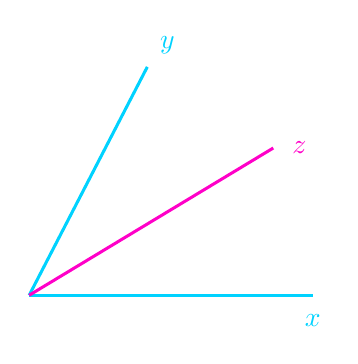
\begin{tikzpicture}[line width=1.1pt]
  \coordinate (O) at (0,0);
  \coordinate (X) at (3.6,0);
  \coordinate (Y) at (1.5,2.9);
  \coordinate (Z) at (3.1,1.87);
  \draw[tmblue] (O) -- (X) node[below=3pt]{$x$};
  \draw[tmblue] (O) -- (Y) node[above right=1pt]{$y$};
  \draw[tmpink] (O) -- (Z) node[right=3pt]{$z$};
\end{tikzpicture}
\end{document}
